\documentclass[journal]{IEEEtran}
\usepackage[spanish]{babel}
\usepackage[utf8]{inputenc}
\usepackage[T1]{fontenc}
\usepackage{graphicx}
\usepackage{amssymb}
\usepackage{amsmath}
\usepackage{amsthm}
\usepackage{booktabs}
\usepackage{gensymb}
\usepackage{stfloats}
\usepackage{float}
\usepackage{nccmath}
%\usepackage{caption}
\usepackage{url}

\title{\textbf{ARMANDO CABLE DIRECTO Y CRUZADO ETHERNET}}

\author{Redes LAN o WAN \\
	\textit{Profesor:} Luis Fernando Díaz Cadavid -  Jaime Alberto Sepúlveda\\ 
	\textit{Monitores:} Juan José Jaramillo Granada - 814034 \\
	Kevin Leonardo Cerpa Campanella - 814017 \\
	Universidad Nacional de Colombia - Sede Manizales}

\date{}

\begin{document}
\maketitle

\section{OBJETIVOS}
\begin{itemize}
\item Analizar los estándares de cableado y los diagramas de pines de Ethernet.
\item Armar un cable directo y un cable cruzado Ethernet.
\item Probar el cable directo y el cable cruzado Ethernet.
 \item Armar una red punto a punto y una red con switches utilizando el cable cruzado y el cable directo Ethernet.
\end{itemize}

\section{DESCRIPCIÓN.}
En esta práctica, analizará los estándares 568-A y 568-B de la Telecommunications Industry Association/Electronic Industries Association (TIA/EIA) y la forma en que se aplican a los cables Ethernet. Luego armará un cable directo y un cable cruzado Ethernet y los probará. Por último, utilizará el cable que acaba de armar para armar una red punto a punto y una red en forma de estrella utilizando un switch.
\section{MATERIALES.}
\begin{itemize}
\item 5 mts de cable UTP categoría 5e como mínimo (Rígido o flexible)
 \item 4 conectores RJ-45 (mínimo).
 \item Tenaza engarzadora RJ-45.
 \item Alicate.
 \item Pelacables.
 \item Comprobador de cables.
 \item 2 PC (Windows).
 \item 1 Switch.
\end{itemize}
\section{ESTÁNDARES DE CABLEADO Y DIAGRAMAS DE PINES DE ETHERNET.}
La TIA/EIA especificó estándares de cableado de par trenzado no blindado (UTP) para el uso en entornos de cableado LAN. Los estándares 568-A y 568-B de la TIA/EIA estipulan los estándares de cableado comercial para las instalaciones de LAN. Estos son los estándares que se utilizan con mayor frecuencia en el cableado LAN de las organizaciones y determinan qué color de hilo se utiliza en cada pin.\\
En un cable directo, los diagramas de pines de ambos extremos se realizan conforme al estándar 568-B (Los 8 hilos (pines) coinciden). Son útiles para conectar dispositivos de red que pertenecen a capas diferentes; por ejemplo, switch con router, PC con switch, router con hub, etc.\\
En un cable cruzado, el segundo y el tercer par del conector RJ-45 en un extremo del cable se invierten en el otro extremo, lo que invierte los pares de envío y recepción. Los diagramas de pines de los cables se realizan conforme al estándar 568-A en un extremo y al estándar 568-B en el otro extremo. Se suelen utilizar para conectar dispositivos de red que pertenecen a la misma capa; por ejemplo, hubs a hubs o switches a switches, pero también se pueden usar para conectar directamente dos hosts, a fin de crear una red simple.\\
\textbf{Nota:} \textit{En los dispositivos de red modernos, a menudo se puede utilizar un cable directo, incluso cuando se conectan dispositivos similares, debido a su característica de detección automática. La detección automática permite a las interfaces detectar si los pares de los circuitos de envío y recepción están conectados correctamente. Si no es así, las interfaces invierten un extremo de la conexión. La detección automática también modifica la velocidad de las interfaces para que coincidan con la más lenta. Por ejemplo, si se conecta una interfaz del router Gigabit Ethernet (1000 Mb/s) a una interfaz del switch Fast Ethernet (100 Mb/s), la conexión utiliza Fast Ethernet.}\\

En la tabla 1(Figura 1) y las figuras 2 y 3, se muestran el esquema de colores y el diagrama de pines, así como la función de los cuatro pares de hilos que se utilizan para el estándar 568-A.

%%%%%%%%%%%
\begin{center}
\begin{figure}[H]
\centering
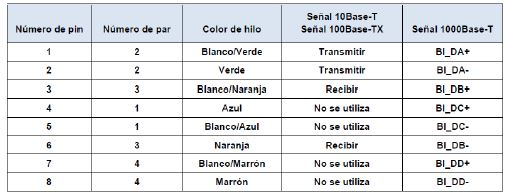
\includegraphics[scale=0.75]{1.JPG} 
\caption{Tabla 1. Ethernet 10/100/1000Base-Tx conforme al estándar 568-A}
\end{figure}
\end{center}
%%%%%%%%%%%%%%%
\begin{center}
\begin{figure}[H]
\centering
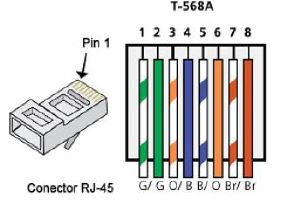
\includegraphics[scale=0.75]{2.JPG} 
\caption{Esquema de colores T-568A}
\end{figure}
\end{center}
%%%%%%%%%%%
\begin{center}
\begin{figure}[H]
\centering
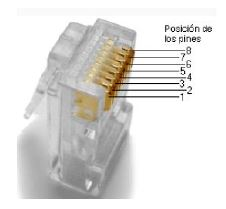
\includegraphics[scale=0.75]{3.JPG} 
\caption{Posición de los pines}
\end{figure}
\end{center}
%%%%%%%%%%%%%%%
En la tabla 2(Figura 4) y la figura 5  , se muestra el esquema de colores y el diagrama de pines conforme al estándar 568-B.
%%%%%%%%%%%
\begin{center}
\begin{figure}[H]
\centering
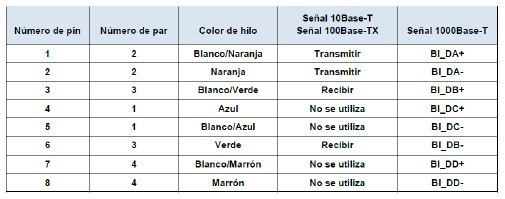
\includegraphics[scale=0.65]{4.JPG} 
\caption{Tabla 2. Ethernet 10/100/1000-BaseTX conforme al estándar 568-B}
\end{figure}
\end{center}
%%%%%%%%%%%%%%%
%%%%%%%%%%%
\begin{center}
\begin{figure}[H]
\centering
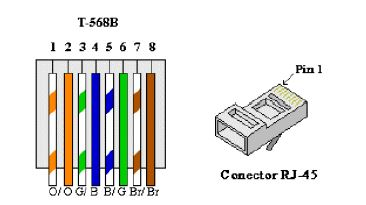
\includegraphics[scale=0.75]{5.JPG} 
\caption{Esquema de colores T-568B}
\end{figure}
\end{center}
%%%%%%%%%%%%%%%
\textbf{Nota 1:}
\textit{En un cable directo los diagramas de pines se realizan conforme al estándar 568-B en ambos extremos.}\\
%%%%%%%%%%%
\begin{center}
\begin{figure}[H]
\centering
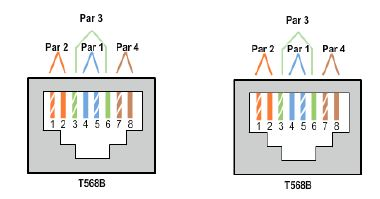
\includegraphics[scale=0.75]{6.JPG} 
\caption{Extremos del cable directo.}
\end{figure}
\end{center}
%%%%%%%%%%%%%%%
\textbf{Nota 2:}
\textit{En un cable cruzado los diagramas de pines de los cables se realizan conforme al estándar 568-A en un extremo y al estándar 568-B en el otro.}
%%%%%%%%%%%
\begin{center}
\begin{figure}[H]
\centering
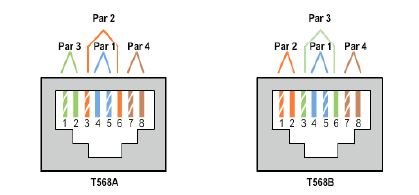
\includegraphics[scale=0.75]{7.JPG} 
\caption{Extremos del cable cruzado.}
\end{figure}
\end{center}
%%%%%%%%%%%%%%%
\section{PROCEDIMIENTO.}
\begin{itemize}
\item Determine la longitud de cable requerida. (3mts)\\
\textbf{Nota:}
\textit{Si estuviera armando un cable en un ambiente de producción, la pauta general indica agregar otros 30,48 cm a la longitud.}
\item Corte un trozo de cable de la longitud deseada y, con un pelacables, retire 5cm aprox. del revestimiento de ambos extremos del cable.
\item Sujete con firmeza los cuatro pares de cables trenzados donde se cortó el revestimiento. Reorganice los pares de cables en el orden que indica el estándar de cableado 568-A o 568-B según sea el caso. Tome todas las precauciones posibles para mantener las torsiones del cable, a fin de proporcionar anulación de ruidos.
\item Aplane, enderece y alinee los hilos con los dedos pulgar e índice.
\item Los hilos de los cables deben estar en el orden correcto conforme al estándar 568-A o 568-B según sea el caso. Utilice el alicate para cortar los cuatro pares en línea recta de 1,25 cm a 2 cm aprox.
\item Coloque un conector RJ-45 en el extremo del cable, con la punta de la parte inferior hacia abajo. Inserte con firmeza los hilos en el conector RJ-45. Todos los hilos se deben poder ver en el extremo del conector en la posición correcta. Si los hilos no se extienden hacia el extremo del conector, retire el cable, vuelva a organizar los hilos según sea necesario y vuelva a insertarlos en el conector RJ-45.
\item Si todo está bien, inserte el conector RJ-45 con el cable en la engarzadora. Engarce con fuerza para que los contactos del conector RJ-45 pasen a través del material aislante de los hilos y, de ese modo, completen el camino conductor. Como en la siguiente figura 8.
%%%%%%%%%%%
\begin{center}
\begin{figure}[H]
\centering
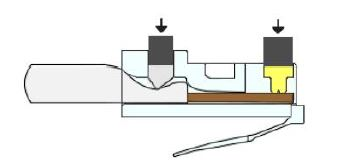
\includegraphics[scale=0.75]{8.JPG} 
\caption{Conector RJ-45.}
\end{figure}
\end{center}
%%%%%%%%%%%%%%%
\item Repita los pasos utilizando el esquema de colores de hilos establecido en el estándar 568-B o 568-B para el otro extremo según sea el caso.
\item Ahora use el comprobador de cables, pruebe el cable cruzado para corroborar la funcionalidad.
\subsection{CONECTAR DOS PC MEDIANTE NIC UTILIZANDO EL CABLE CRUZADO ETHERNET:}
%%%%%%%%%%%
\begin{center}
\begin{figure}[H]
\centering
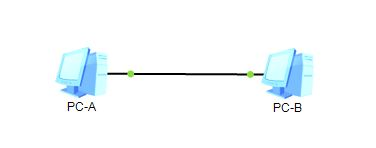
\includegraphics[scale=0.75]{9.JPG} 
\caption{Red punto a punto.}
\end{figure}
\end{center}
%%%%%%%%%%%%%%%

\item Realice un ping a la misma tarjeta de red del equipo a la dirección de red 127.0.0.0/255.0.0.0 para comprobar que se encuentra funcionando adecuadamente el protocolo TCP/IP en el PC.
\item Configure la dirección IP de ambas PCs de manera que correspondan a la misma subred.\
Por ejemplo, si la PC es la PC-A, la dirección IP debe configurarse en 192.168.10.1 con una máscara de subred de 24 bits, entonces la dirección IP de la PC-B debe ser 192.168.10.2.\
La dirección de gateway predeterminado puede dejarse en blanco.
\item Utilice el cable cruzado que armó y conecte las dos PC con las NIC.
\item En el símbolo del sistema (cmd) de la PC-A, haga ping a la dirección IP de la PC-B, repita el proceso pero de la PC-B a la PC-A.\\
\textbf{Nota:}
\textit{Es posible que el Firewall de Windows tenga que deshabilitarse temporalmente para que los pings sean correctos. Si el firewall se deshabilita, vuelva a habilitarlo al final de esta práctica de laboratorio.}

\subsection{COMPARTIR CARPETAS Y ARCHIVOS EN RED}
Después de conectar dos PCs y probar conectividad entre ellos usando el comando ping:
\item Ingrese a “Mis sitios de red” y luego a “Ver equipos del grupo de trabajo”; y
aparecerá la lista de recursos compartidos del PC (carpetas, impresoras, etc). Podrá ver lo que se encuentra en ese PC y modificar lo que sea posible, así como copiar archivos desde dichas carpetas a su computador, o viceversa.\\
\textbf{Nota:}
\textit{Se puede compartir cualquier carpeta o incluso una unidad de disco completa, sim-plemente, usando el botón derecho del ratón sobre dicho elemento, y eligiendo "Compar-tir". Es posible darle un nombre a la carpeta compartida, personalizarla y elegir el tipo de acceso:}\\
\textbf{Sólo lectura:}
\textit{ Los demás usuarios de la red podrán leer el contenido de la carpeta, e in-cluso copiarlo a sus PCs, pero no borrarlo, modificarlo, crear nuevos archivos o carpetas dentro.}\\
\textbf{Oculto:}
\textit{El archivo no podrá ser visible a menos que se habilite la opción de ver archivos ocultos en el equipo.}\\
\item  Las acciones disponibles para realizar en las propiedades de la carpeta que se desea compartir cambian dependiendo de si está o no habilitada la opción “Utilizar uso compar-tido simple de archivos”, la cual está en el menú de “Opciones de carpeta” en las Herra-mientas del sistema.
%%%%%%%%%%%
\begin{center}
\begin{figure}[H]
\centering
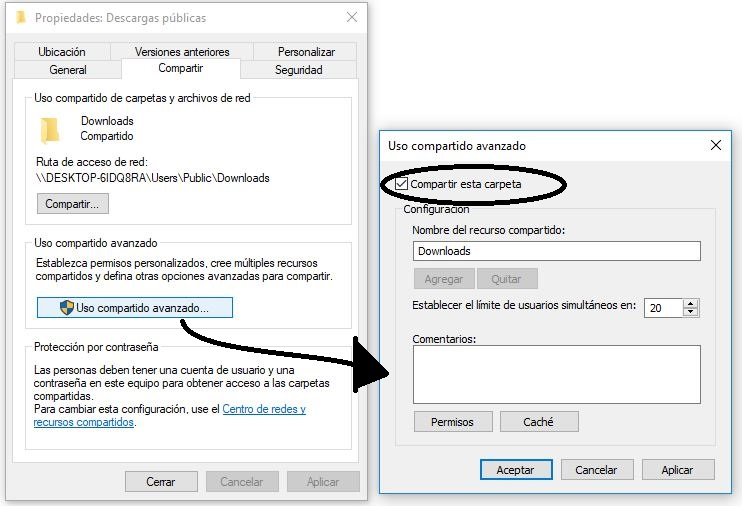
\includegraphics[scale=0.5]{10.JPG} 
\caption{Propiedades para compartir una carpeta en la red.}
\end{figure}
\end{center}
%%%%%%%%%%%%%%%
Otra manera de ingresar al entorno compartido del otro computador es a través de la op-ción “Ejecutar”, que se encuentra en el menú Inicio. Escriba la dirección IP del PC. Por ejemplo \textbackslash{}\textbackslash{}:192.168.0.1.\\
\item Para visualizar y administrar las carpetas que se encuentran compartidas en el PC, se
ingresa al Panel de Control y se selecciona “Herramientas administrativas”, después entra-mos al ícono que se llama “Administración de equipos” y desde allí ya podemos mirar las carpetas que están compartidas y administrar las cuentas de usuarios.
\subsection{COMPARTIR CARPETAS Y ARCHIVOS EN RED CON SWITCHES}.
\item Conecte uno o más computadores por medio de un cable directo a un switch para formar una red en estrella, debe hacerse a través de las tarjetas Ethernet
%%%%%%%%%%%
\begin{center}
\begin{figure}[H]
\centering
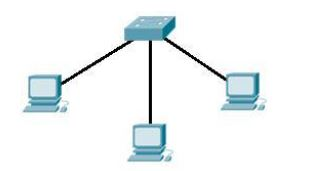
\includegraphics[scale=0.75]{11.JPG} 
\caption{Red en estrella}
\end{figure}
\end{center}
%%%%%%%%%%%%%%%
\item Utilice el protocolo TCP/IP, de forma que las direcciones IP de los PCs tengan la misma máscara de subred para que sea posible la comunicación entre ellos.\\
\item Escoja un nombre de hasta 15 caracteres para la red (evite el uso de espacios, acentos y eñes).\\
\item Realice un ping a cada uno de los computadores conectados al switch para verificar la conexión.\\
\item  Vuelva al literal a. de la sección “COMPARTIR CARPETAS Y ARCHIVOS EN RED” de esta guía y empiece a intercambiar información con cada uno de los PCs conectados al switch.
\end{itemize}
\end{document}

